\documentclass{beamer}
\usefonttheme[onlymath]{serif}

\usepackage{amsfonts}

% Code Block Setting
\usepackage{listings}
\lstset{language=C,
numberstyle=\footnotesize,
basicstyle=\ttfamily\footnotesize,
numbers=left,
stepnumber=1,
frame=shadowbox,
breaklines=true}

\usetheme{Warsaw}
% \usecolortheme{dove}

% Add frame number and total frame number in footline
\defbeamertemplate*{footline}{shadow theme}{%
    \leavevmode%
    \hbox{\begin{beamercolorbox}[wd=.5\paperwidth,ht=2.5ex,dp=1.125ex,leftskip=.3cm plus1fil,rightskip=.3cm]{author in head/foot}%
            \usebeamerfont{author in head/foot}\hfill\insertshortauthor
        \end{beamercolorbox}%
        \begin{beamercolorbox}[wd=.4\paperwidth,ht=2.5ex,dp=1.125ex,leftskip=.3cm,rightskip=.3cm plus1fil]{title in head/foot}%
            \usebeamerfont{title in head/foot}\insertshorttitle\hfill%
        \end{beamercolorbox}%
        \begin{beamercolorbox}[wd=.1\paperwidth,ht=2.5ex,dp=1.125ex,leftskip=.3cm,rightskip=.3cm plus1fil]{title in head/foot}%
            \hfill\insertframenumber\,/\,\inserttotalframenumber
    \end{beamercolorbox}}%
    \vskip0pt%
}

% Tikz related
\usepackage{tikz}
\usetikzlibrary{fit}
\usetikzlibrary{calc}
\usetikzlibrary{positioning}

% Number the figures
\setbeamertemplate{caption}[numbered]

% Add outline page at begining of each section
\AtBeginSection[]
{
    \begin{frame}<beamer>
        \frametitle{Outline}
        \tableofcontents[currentsection, hideallsubsections]
    \end{frame}
}

%%%%%%%%%%%%%%%%%%%%%%%%%%%%%%%%%%%%%%%%%%%%%

\title{High-performance Energy-efficient Recursive Dynamic Programming with Matrix-multiplication-like Flexible Kernels}
\author{
    Jesmin Jahan Tithi\inst{1},\\
    Pramod Ganapathi \inst{1},\\
    Sonal Aggarwal\inst{1},\\
    Rezaul Chowdhury\inst{1}
}
\institute{
    \inst{1} Department of Computer Science, Stony Brook University, New York, 11790-4400, USA
}
\date{
    \tiny{2015 IEEE 29th International Parallel and Distributed Processing Symposium}\\
    \tiny{Presented by ShiangYun Yang}
}

\begin{document}
\begin{frame}
    \titlepage
\end{frame}

\section{Introduction}

\subsection{Sparse Matrix Vector Multiplication}
\begin{frame}
    \frametitle{Definition and Propety}
	\begin{itemize}
		\item A sparse matrix is a matrix in which most of the elements 
			are zero.
		\item Sparse data is by nature more easily compressed and thus 
			require significantly less storage.
			\begin{itemize}
				\item Many formats have been proposed, such as CSR, 
					CRS, DIL, and so on.
			\end{itemize}
	\end{itemize}
\end{frame}

\subsection{CSR Format}
\begin{frame}[fragile]
	\frametitle{Compressed Row Storage}
	\begin{align*}
		A = \begin{bmatrix}
			0 & 0 & a & 0 & 0 & 0 & b & c \\
			0 & 0 & d & e & 0 & 0 & f & 0 \\
			0 & 0 & 0 & 0 & g & h & i & j \\
			k & l & 0 & 0 & m & n & o & p \\
		\end{bmatrix}
	\end{align*}
	\begin{table}[]
		\centering
		\caption{CSR format}
		\label{my-label}
		\begin{tabular}{l | c | c | c | c | c | c | c}
			\hline
		index & 0 & 1 & 2 & $\cdots$ & 12 & 13 & 14 \\ \hline
		val      & a & b & c & $\cdots$ & m & n & p  \\ \hline
		col\_ind & 2 & 6 & 7 & $\cdots$ & 4 & 5 & 7 \\ \hline
		\end{tabular}
		\\
		\begin{tabular}{l | c | c | c | c | c}
			\hline
		rowptr      & 0 & 3 & 6 & 10 & 15 \\ \hline
		\end{tabular}
	\end{table}
\end{frame}

\subsection{Serial Implementation Example}
\begin{frame}[fragile]
	\frametitle{Serial Implementation Example}
	\begin{itemize}
		\item $A_{n,m} \times x_{m,1} = y_{n,1}$
\begin{lstlisting}
for (i = 0; i < n; ++i) {
    double y0 = y[i];
    for (k = rowptr[i]; k < rowptr[i+1]; ++k)
        y0 += val[k] * x[column_index[k]];
    y[i] = y0;
}
\end{lstlisting}
	\end{itemize}
\end{frame}

\subsection{Changes of Parallel Implementation}
\begin{frame}
	\frametitle{Changes of Parallel Implementation}
	\begin{itemize}
		\item Bandwith
			\begin{itemize}
				\item the upper bound of $\text{FLOPS}\footnote{Floating-Point Operations Per Second }:\text{BYTES} = 0.25$
			\end{itemize}
		\item Load imbalance
			\begin{itemize}
				\item The non-zeros in a matrix may not be evenly distributed 
					across different rows.
				\item The matrix data have low reuse. Each non-zero element 
					is only once for computing the corresponeding dot product.
			\end{itemize}
	\end{itemize}
\end{frame}

\subsection{Executive Summary}
\begin{frame}
	\frametitle{Executive Summary}
	\begin{itemize}
		\item Improve the bandwidth by block-based compressed common
			coordinate format.
		\item Addressing the load imbalance problem by customized
			efficient segmented scan/sum.
		\item Using auto-tuning framework to explore optimization parameter 
			for different sparse matrices and different platforms.
	\end{itemize}
\end{frame}


\section{Algorithm}

\subsection{Constraint Condition}
\begin{frame}
    \frametitle{Constraint Condition}
    \begin{itemize}
		\item Assume $n = 2^t$ for some integer $t \ge 0$ for all problems.
		\item The size of DP table is $n \times n$.
	\end{itemize}
\end{frame}

\subsection{Parenthesization Problem}
\begin{frame}
    \frametitle{Parenthesization Problem}
    \begin{figure}
		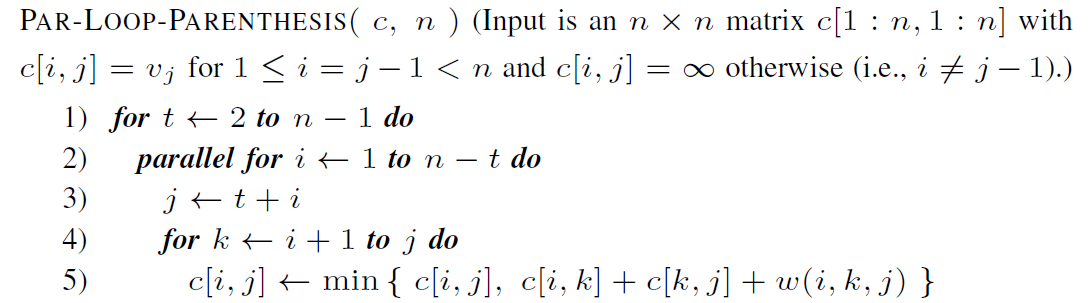
\includegraphics[scale=0.4]{figure/fig-parenthesis.png}
	\end{figure}
    \begin{itemize}
    	\item $w(i, k, j)$ returns the cost of combining parenthesizations of
    		$x_i \; \cdots x_k$ and $x_k \; \cdots x_j$
    	\item The optimal parenthesizing cost $c[1, n]$ for the entire sequence.
    \end{itemize}
\end{frame}

\subsection{Parenthesization Problem - Parallel CORDAC}
\begin{frame}
    \frametitle{Parallel CORDAC Algorithm - Func A, B}
    \begin{figure}
		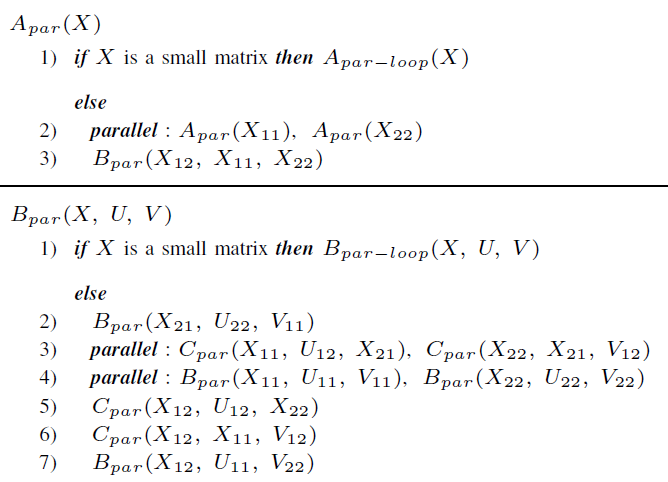
\includegraphics[scale=0.5]{figure/fig-parenthesis-parallel-1.png}
	\end{figure}
\end{frame}

\begin{frame}
    \frametitle{Parallel CORDAC Algorithm - Func C}
    \begin{figure}
		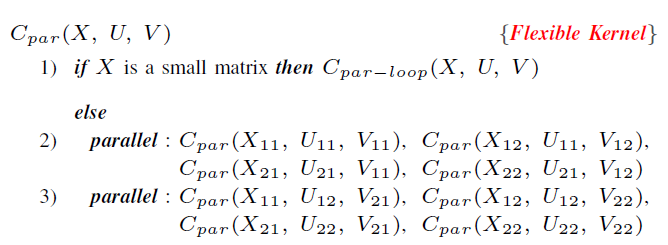
\includegraphics[scale=0.5]{figure/fig-parenthesis-parallel-2.png}
	\end{figure}
\end{frame}

\begin{frame}
    \frametitle{Parallel CORDAC Algorithm Figure}
    \begin{figure}
        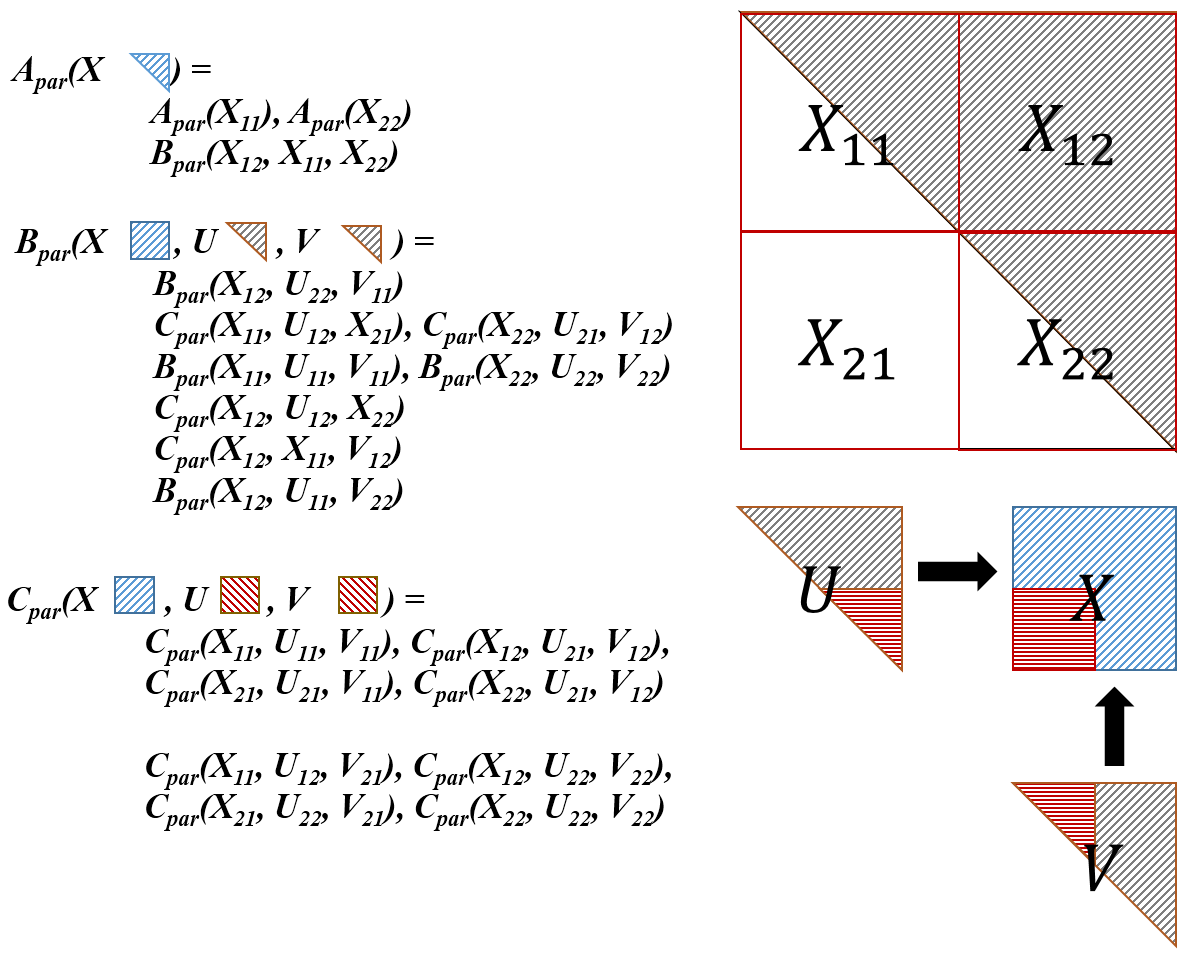
\includegraphics[scale=0.25]{figure/fig-par-explain.png}
    \end{figure}
\end{frame}

\subsection{Other Problems}
\begin{frame}
    \frametitle{Other Problems}
    \begin{figure}
		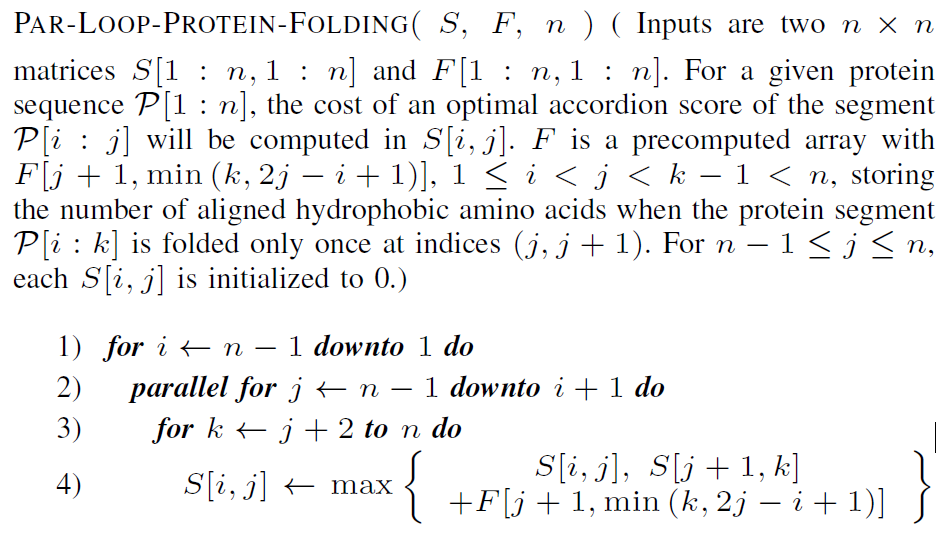
\includegraphics[scale=0.2]{figure/fig-folding.png}
	\end{figure}
	\begin{figure}
		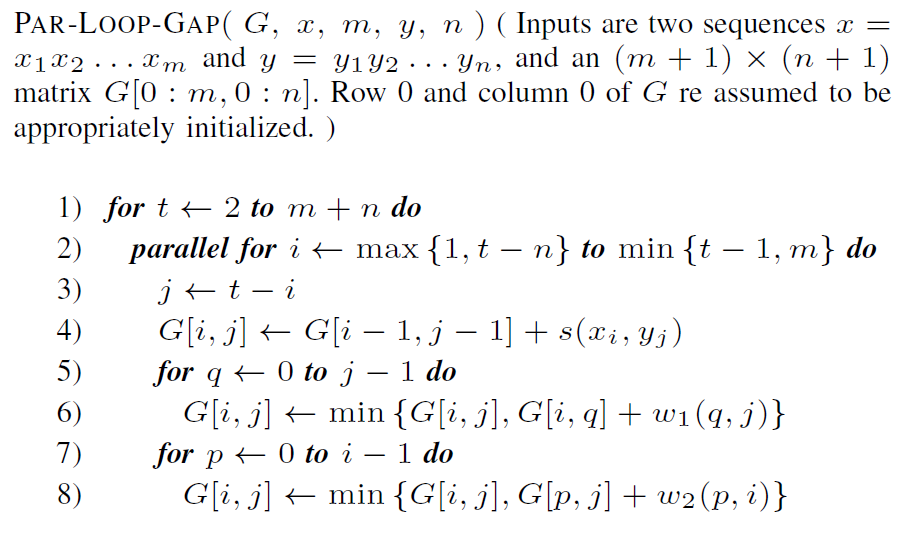
\includegraphics[scale=0.2]{figure/fig-gap.png}
	\end{figure}
\end{frame}

\subsection{Other Problems - Parallel CORDAC}
\begin{frame}
    \frametitle{Other Problems - Parallel CORDAC}
    \begin{figure}
		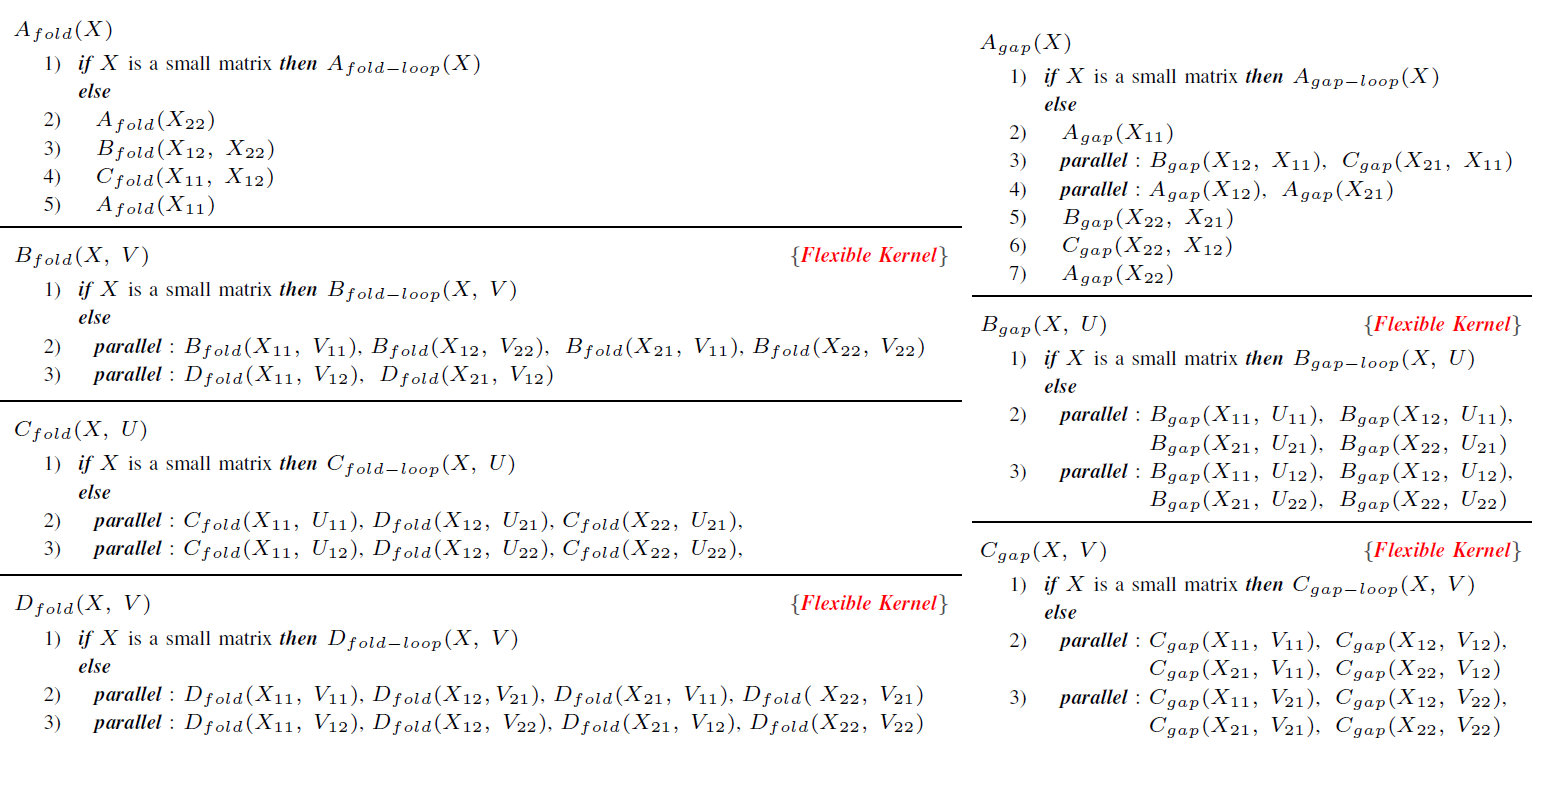
\includegraphics[scale=0.2]{figure/fig-fold-gap-parallel.png}
	\end{figure}
\end{frame}

\begin{frame}
    \frametitle{Other Problems - Parallel CORDAC}
    \begin{figure}
		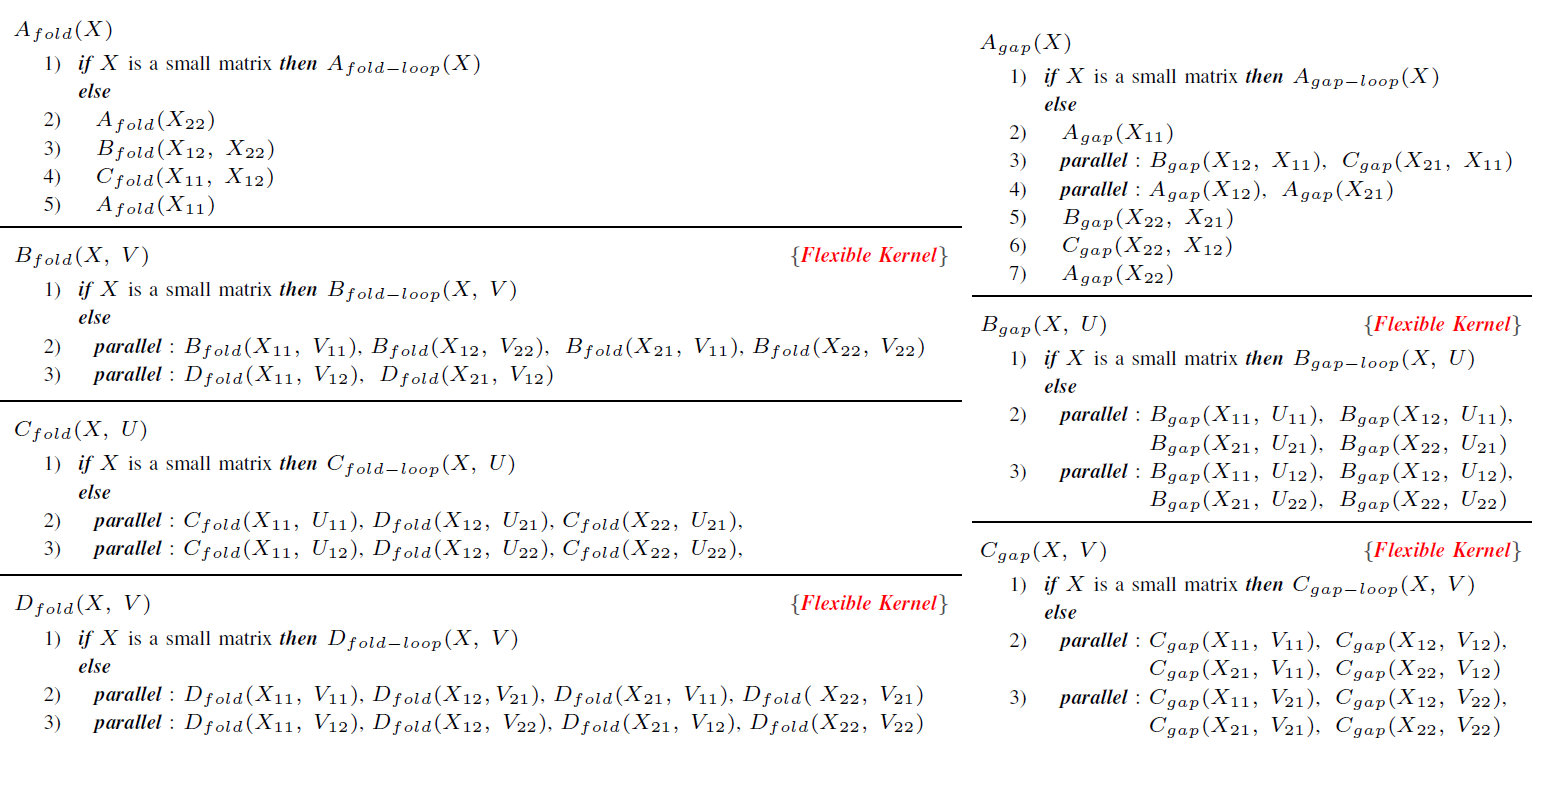
\includegraphics[scale=0.2]{figure/fig-fold-gap-parallel.png}
	\end{figure}
\end{frame}
\section{Complexity Analysis}

\subsection{Complexity Analysis}
\begin{frame}
    \frametitle{Complexity Analysis}
    \begin{figure}
		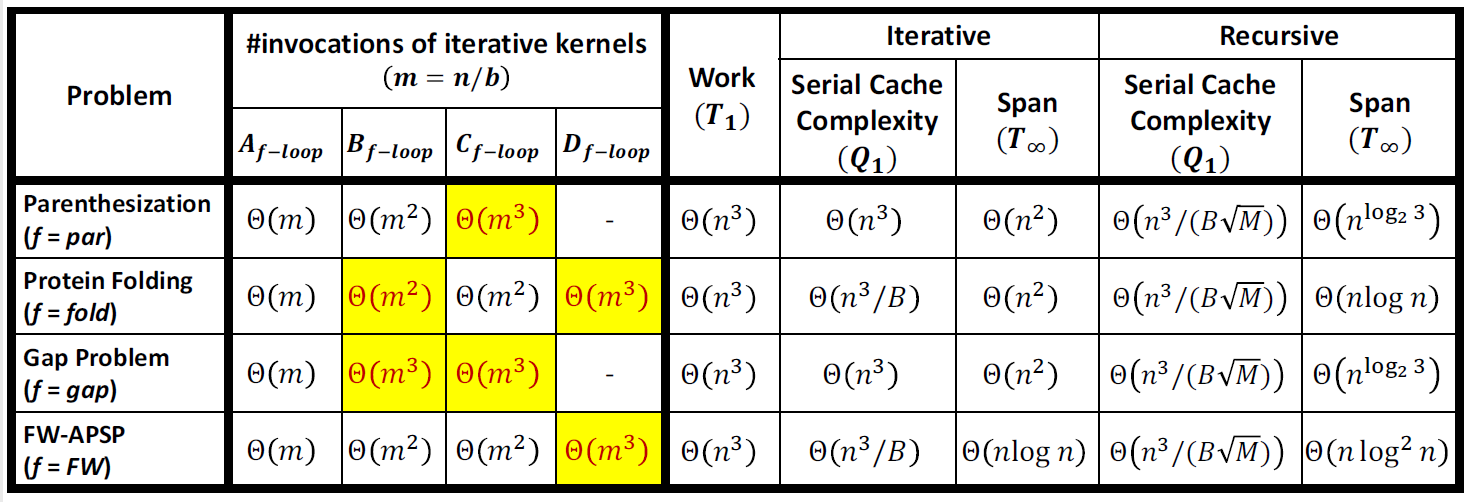
\includegraphics[scale=0.25]{figure/fig-complexity.png}
	\end{figure}
    \begin{itemize}
		\item size of cache $M$, cache line size $B$, processing elements $p$
		\item Runtime $T_p = \mathcal{O}(T_1/p + T_{\infty})$
		\item Cache complexity $Q_p = \mathcal{O}(Q_1 + p(M/B) T_{\infty})$
	\end{itemize}
\end{frame}
\section{Optimization}

\subsection{Hybrid CORDAC}
\begin{frame}
    \frametitle{Hybrid CORDAC}
    	It retain the benefits of both iterative and recursive algorithms.
		Cache-efficient algorithm recursive subdivision continues until 
		the problem size becomes small enough.
	\begin{itemize}
		\item Asymptotic Improvement in Parallelism
		\item Highly Optimizable Base Cases
	\end{itemize}
\end{frame}

\subsection{Optimizing Kernel Functions}
\begin{frame}
    \frametitle{Optimizing Kernel Functions}
	Inside flexible kernel, 
	\begin{itemize}
		\item Copy-optimization: Copy the data into local $b \times b$ 
			static arrays.
		\item Loop Reordering: It is possible to change
			the looping order without hampering the correctness of the algorithms.
	\end{itemize}
\end{frame}

\subsection{Data Layout}
\begin{frame}
    \frametitle{Data Layout}
	\begin{figure}
		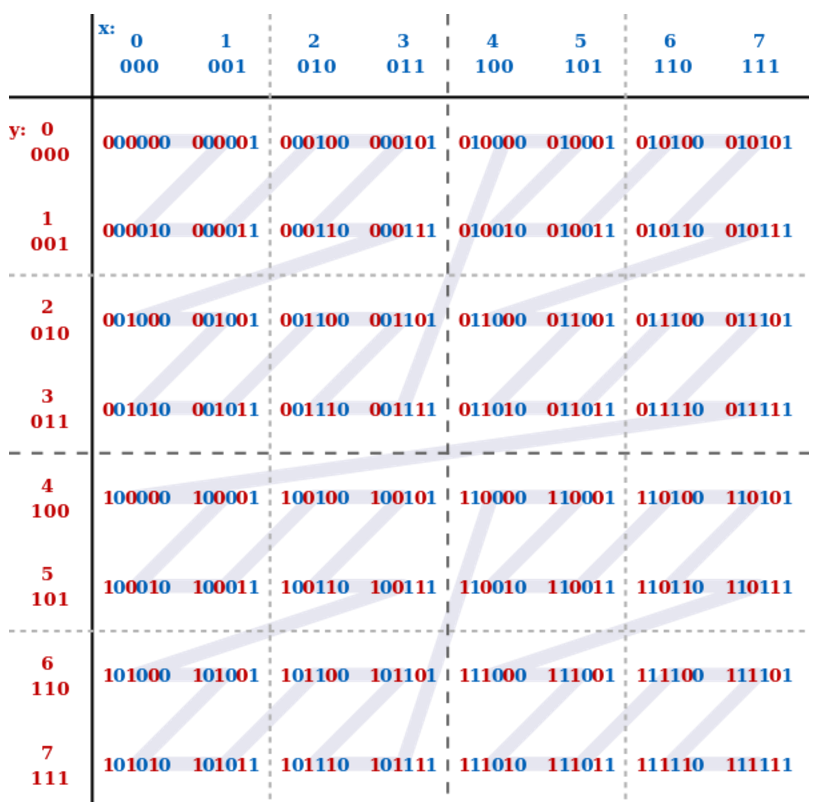
\includegraphics[scale=0.2]{figure/fig-z-morton.png}
	\end{figure}
	\begin{description}
		\item[Z-Morton Row-Major] ZM\_RM layout improves both temporal and 
			spatial localities.
	\end{description}
\end{frame}

\subsection{Auto vs. Explicit Vectorization}
\begin{frame}
    \frametitle{Auto vs. Explicit Vectorization}
	\begin{itemize}
		\item It often vectorize the base-case of the dominating kernel. 
		\item For example, $C_{\textit{loop}}$ is enough to get the 
			major share of the speedup.
	\end{itemize}
\end{frame}

\section{Experiment}

\subsection{Configuration}
\begin{frame}
    \frametitle{Configuration}
    \begin{itemize}
    	\item Four versions
		    \begin{itemize}
				\item \textit{LOOPDP}: optimized looping code with padding
					to mitigate set-associativity problem.
				\item \textit{CO}: unoptimized CORDAC.
				\item \textit{CO\_Opt}: optimized CORDAC + copy-optimization.
				\item \textit{COZ}: \textit{CO\_Opt} + \textit{ZM\_RM} 
					layout for data storage.
			\end{itemize}
		\item Base-case size of $64 \times 64$ for parenthesis, gap and protein 
			folding and $128 \times 128$ for FW-APSP.
	\end{itemize}
\end{frame}

\subsection{Platforms}
\begin{frame}
    \frametitle{Platforms}
    \begin{figure}
		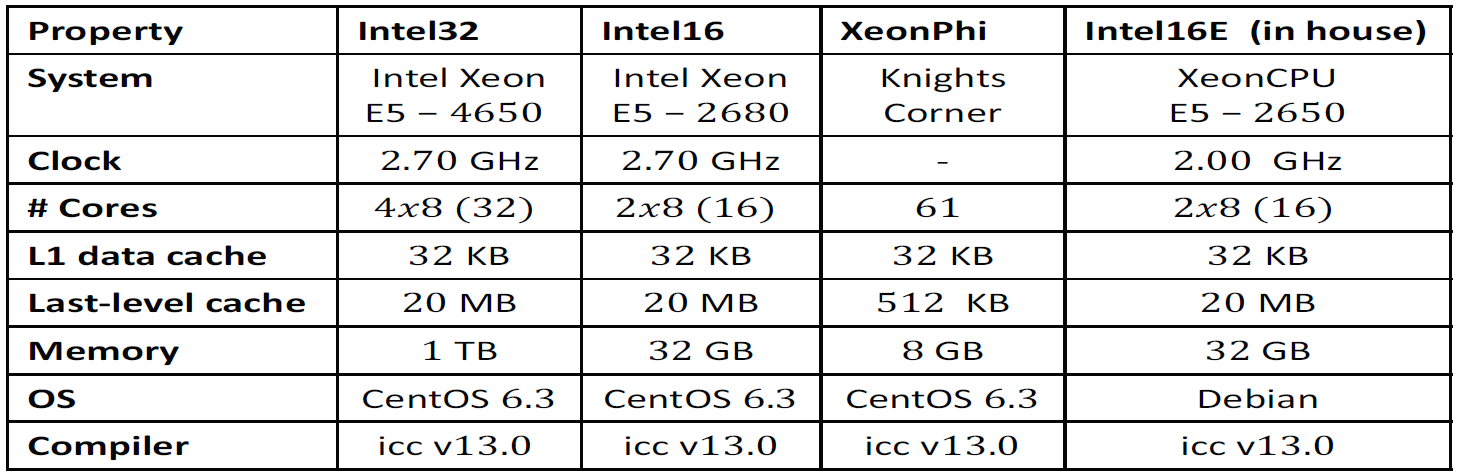
\includegraphics[scale=0.3]{figure/fig-platforms.png}
	\end{figure}
\end{frame}

\subsection{Shared-Memory Machine}
\begin{frame}
    \frametitle{Performance on Shared-Memory Machine}
    \begin{itemize}
    	\item For parenthesization problem, hybrid CPU + 
    		Xeon Phi version runs $395\times$ for $n = 32768$.
    	\item Explicit vectorization contributed up to $5\times$ speedup
    		over auto-vectorized code.
    	\item CORDAC algorithms consume $4$ -- $30\times$ less energy.
    \end{itemize}
\end{frame}

\begin{frame}
    \begin{figure}
		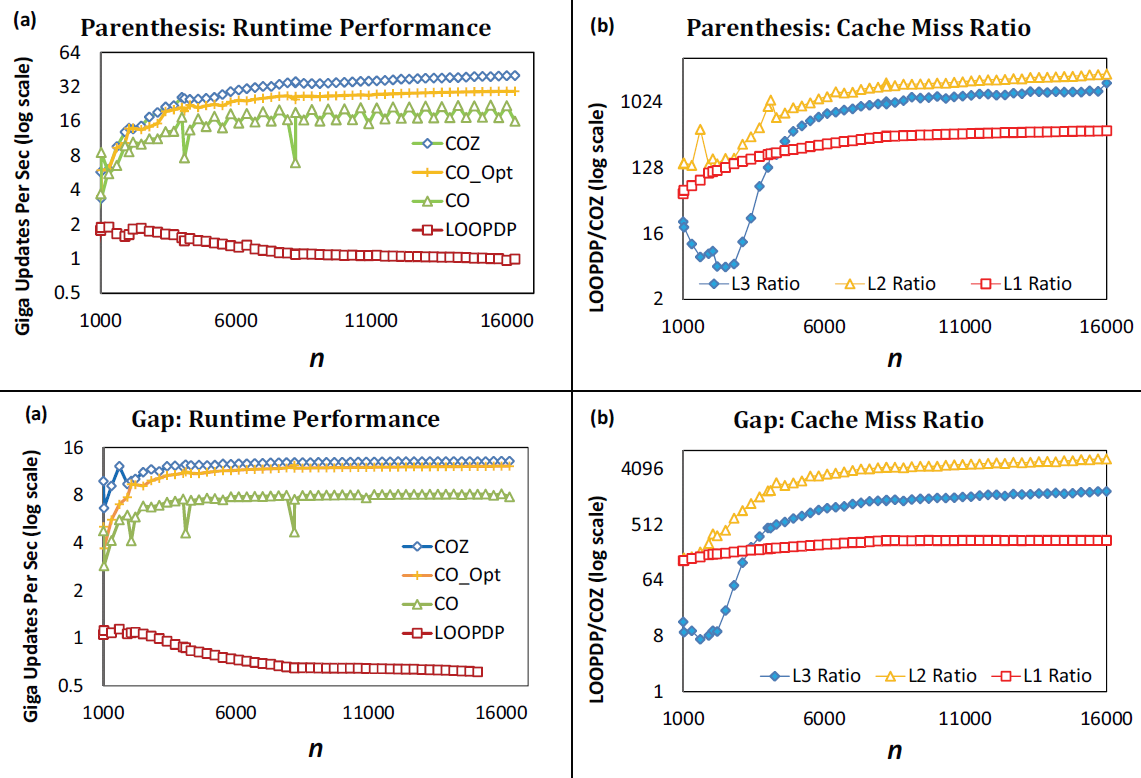
\includegraphics[scale=0.3]{figure/fig-shared-machine-1.png}
	\end{figure}
	\footnote{Performance on Intel 16: Intel Xeon E5-2680}
\end{frame}

\begin{frame}
    \begin{figure}
		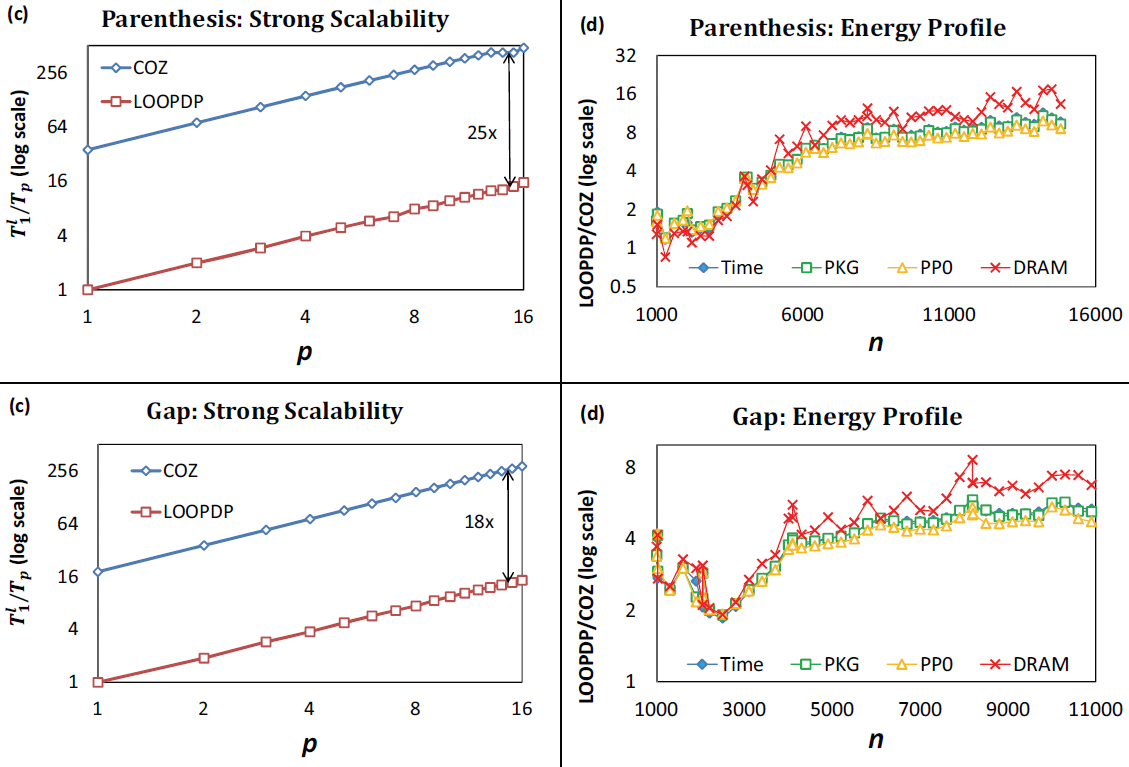
\includegraphics[scale=0.3]{figure/fig-shared-machine-2.png}
	\end{figure}
	\footnote{Performance on Intel 16: Intel Xeon E5-2680}
\end{frame}

\section{Extension to Distributed Memory}

\subsection{SDSM Framework Introduction}
\begin{frame}
    \frametitle{SDSM Framework}
    	This paper propose a novel shared-distributed-shared-memory (SDSM) 
    	framework for our CORDAC algorithms. They use
    \begin{itemize}
    	\item Hierarchical dynamic load-balancing,
    	\item Work-stealing
    \end{itemize}
     	to balance the load among the processes.
\end{frame}

\subsection{SDSM: Multi-level Hierarchy}
\begin{frame}
    \frametitle{Multi-level Hierarchy}
    If we have $K$ processes,
    \begin{itemize}
    	\item a super-master,
    	\item some $M'$ of them as masters, and
    	\item the rest as workers.
    \end{itemize}
    They run multithreaded code on $p$ cores.
\end{frame}

\begin{frame}
    \frametitle{Shared Job Queue}
    \begin{itemize}
    	\item Each super-master/master process maintains a shared 
    		job queue.
    	\item If a thread run a function on input size $x$ 
    		($\textit{min offload threshold} \le x \le \textit{max offload threshold}$), 
    		try to lock the job queue and put at most $l-1$
    		out of its $l$ parallellly executable recursive sub-divisions in job queue.
    	\item If a thread waits its submitted jobs finished,
    		it steals back its latest submitted jobs left in the job queue.
    \end{itemize}
\end{frame}

\subsection{SDSM: Result}
\begin{frame}
    \frametitle{Result}
    \begin{figure}
		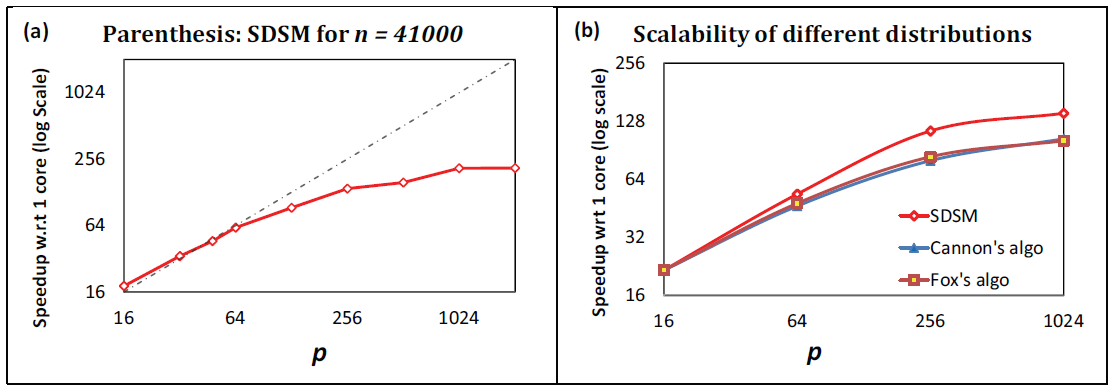
\includegraphics[scale=0.3]{figure/fig-distributed-result.png}
	\end{figure}
    \begin{itemize}
    	\item For parenthesization problem, we fixed $n$ at $41 K$ and 
    		allowed offloading of problems with a size in the range of
    		$256$ -- $2048$.
    \end{itemize}
\end{frame}

\end{document}
